\chapter{Objective Assessment}
\label{chap:objective}
This chapter contains the development process of the Face Quality Analysis application. To start we will look at functional and non-functional requirements followed by use cases. Further, we include sequence diagrams to show how some of the core functionality work. To the end we will have an insight in the design and implementations phase.

\section{Requirements}
\label{sec:requirements}
When approaching the requirements, we had to make decisions based on the task description as well as the meetings with Mobai. The description and our colleagues were open in terms of setting requirements, but some core concepts of the desired product were simplicity, clarity, performance and modifiability. Based on these principles, we along with Mobai shaped non-functional and functional requirements. Also, as mentioned in Section \ref{sec:OurModel} not all requirements were set at the start of the project, so they had to be fine-tuned and confirmed along the development process. This did not mean that any important change in the software occurred, but as more functionality were suggested, requirements had to be created to describe them. The \textbf{non-functional} requirements describes how the software should perform. These are the following requirements:
\begin{itemize}
    \item The application should be deployed in a container.
    \item The architecture should consist of a backend and a frontend.
    \item APIs should be implemented as REST APIs.
    \item The application should make it easy to add new FIQMs.
\end{itemize}
The \textbf{functional} requirements defines what the software should do or not do. These are the following requirements:
\begin{itemize}
    \item The application should run every available FIQM separately.
    \item The application should run all FIQMs together.
    \item The application should return a sheet with quality scores on every image based on the FIQMs as a JSON file.
    \item If only one image is evaluated, the image should be displayed with corresponding attribute scores. 
\end{itemize}

\subsection{What type of application}
The responsibility of choosing application type was given to the bachelor group. Selecting either a web or desktop application was challenging, but we carefully evaluated the type of application that suited our needs the best. 

\subsubsection*{Desktop application}
Since desktop applications are downloaded to your operating system, they are available independently whether you are connected to the internet or not. In that way it is possible to stay functional all the time \cite{WebVsDesktop}. The constant accessibility that desktop applications provide automatically make them more secure. In a way, you never have to be connected to the internet when working on tasks which reduces the possibility of being hacked by a margin. Having a fast computer would be beneficial running a desktop application. The application uses memory and CPU which returns a good user experience given a resourceful computer. However, using an old computer would not be a problem either. The fact that desktop applications allows for running older versions of the program with all functional availability does not make a hardware upgrade necessary. Also, given that desktop applications do not coerce to update, the software makes it adaptable to choose a suitable version for the computer's specifications. It is also uncomplicated to store files from the application, as information are supported by the computer's hard drives. 

Although, desktop applications have their downsides. The application may require multiple updates to enable full functionality which seems persistent and unnecessary. If the work is performed on different devices, each device need the same installation to synchronize the progress. This will also make it more challenging for multiple users to collaborate on desktop applications. Another disadvantage with a desktop application is the dependence of operating system requirements. To allow the latest functionality the application provides, specific requirements are required. 

\subsection*{Web application}
A web application only require one installation step before the software is workable \cite{WebVsDesktop}. This is time saving because the only thing to do is to type the internet address into the browser. All updates are free and immediately available. The ease of availability for these applications make synchronizing with several devices a small case. In addition to this, the simplicity of managing cooperation with different users is remarkable. Some licence issues may arise, but this solution makes people collaborate from their permanent working stations. Another advantage is the application's accessibility. It is possible to acquire web applications from any browser or operating system. 

However, web applications do not offer offline mode which requires a constant internet connection. In addition, the application's capability depends on the internet connection and speed. A poor connection and speed result in a bad workflow. As regular updates could be beneficial, there are less possibilities of using older versions of the software. 

\subsection*{Our application}
We chose to build a web application as our approach. Given the intuitive user interface with a limited amount of functions, it was easier and more meaningful to develop a web application. We felt a desktop application would be more suitable if the application requirements increased and the programming tasks were more complex. Our web application would be time saving and comprehensible for Mobai employers since the application only need one installation before working on the software. When new FIQMs are integrated to the applications, the update is uncomplicated and users can instantly evaluate facial images with the new incoming metrics. 

%We chose to build a web application as our approach. Mobai did not need to run the application in offline mode, since they always had sufficient internet connection. Also, because many employers would work on the web page at the same time, it should be easy to manage multiple users so they can work on their required working stations.% 

\section{Use case}
We have created a use case diagram to show the core functionality and activities within the application. The diagram was built from the perspective of the user (described in Section \ref{sec:TargetGroups}) which were employees at Mobai. The cases differ in complexity where running all metrics would be the most challenging. That is because it includes running every metric and providing scores for each image. 

\begin{figure}[h]
    \centering
    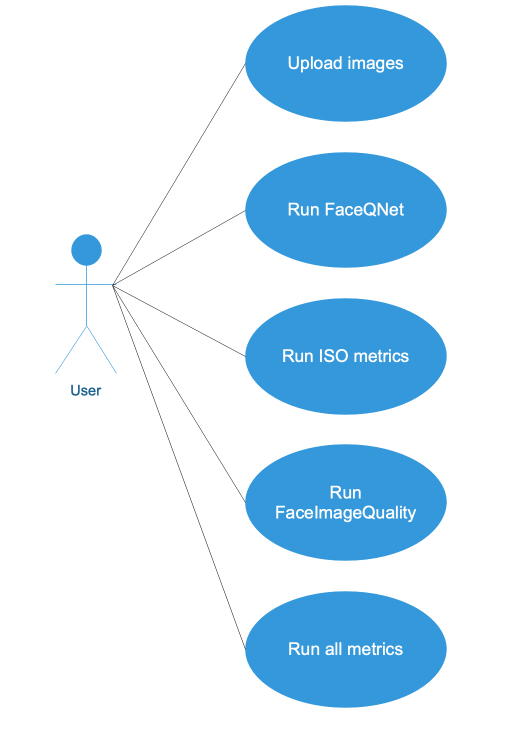
\includegraphics[scale = 0.4]{figures/UseCaseDiagram.png}
    \caption{Use case diagram}
    \label{fig:UseCase}
\end{figure}

\newpage

\begin{table}[h]
\centering
\resizebox{\textwidth}{!}{%
\begin{tabular}{|p{12cm}|} 
\hline
\textbf{Use case:} Upload images\\
\textbf{Actor:} User \\
\textbf{Goal:} Upload selected images \\
\textbf{Description:} The user can select what images he would like to upload to the application. Images will only be stored in the application in that session. \\ \hline
\end{tabular}%
}
\end{table}


\begin{table}[h]
\centering
\resizebox{\textwidth}{!}{%
\begin{tabular}{|p{12cm}|} 
\hline
\textbf{Use case:} Run ISO metrics\\
\textbf{Actor:} User \\
\textbf{Goal:} Evaluate images with the ISO metric \\
\textbf{Description:} After uploading selected images, the user would press ''Run ISO metrics'' to assess the images. The application returns a sheet with quality scores for each facial image. \\ \hline
\end{tabular}%
}
\end{table}

\begin{table}[h]
\centering
\resizebox{\textwidth}{!}{%
\begin{tabular}{|p{12cm}|} 
\hline
\textbf{Use case:} Run FaceQnet\\
\textbf{Actor:} User \\
\textbf{Goal:} Evaluate images with the FaceQnet \\
\textbf{Description:} After uploading selected images, the user would press ''Run FaceQnet'' to assess the images. The application returns a sheet with quality scores for each facial image. \\ \hline
\end{tabular}%
}
\end{table}


\begin{table}[H]
\centering
\resizebox{\textwidth}{!}{%
\begin{tabular}{|p{12cm}|} 
\hline
\textbf{Use case:} Delete images\\
\textbf{Actor:} User \\
\textbf{Goal:} Remove images from the session \\
\textbf{Description:} After running the metrics on the uploaded images, the user is able to remove all images used that session. \\ \hline
\end{tabular}%
}
\end{table}


\begin{table}[h]
\centering
\caption{High level use case for ``Run all metrics''}
\resizebox{\textwidth}{!}{%
\begin{tabular}{|l|p{9cm}|} 
\hline
\textbf{Case} & Run all metrics  \\ \hline
\textbf{Description} & The user runs all metrics in the application which returns scores for every image.      \\ \hline
\textbf{Basic Flow} &   \begin{enumerate}
    \item The user presses the ``upload images'' button.
    \item The user navigates to select wanted images to execute the metrics on.
    \item After uploading images, the user presses ``Run all metrics''
    \item The program returns a sheet with quality scores of the selected images
\end{enumerate}     \\ \hline
\textbf{Alternative} &  The user runs all metrics without uploading any images
            \begin{enumerate}
                \item The application displays an error and asks the user to upload images.
            \end{enumerate}
The user presses reset before running the metrics 
            \begin{enumerate}
                \item Uploading images again is necessary.
            \end{enumerate}
                    \\  \hline
\textbf{Pre-condition} & The application is running and images are uploaded. \\ \hline
\textbf{Post-condition} &  The FIQMs have predicted the perceived face quality on the images. \\ \hline
\end{tabular}%
}
\end{table}

\clearpage


\section{Choice of front- and backend}
When choosing development software, we had to take some considerations. First, both backend and frontend software should not be time consuming to master, given that the project consisted of coding and research. Second, it should be uncomplicated to integrate the released FIQMs with the backend as well as creating an intelligible user interface. 

\subsection*{Backend}
The two FIQMs FaceQnet and ISO metrics were written in Python. Since we were experienced with Python and operated with it in courses throughout the bachelor program, it was natural to choose a Python framework for the backend. With a dozen of possible web frameworks, we needed to select a framework which suited our needs in terms of scalability, performance and ease of use. In the end, the choices were between Django and Flask. 

\newpage

\begin{table}[h]
\centering
\caption{Pros and cons with Django}
\resizebox{0.9\textwidth}{!}{%
\begin{tabular}{|l|p{9cm}|} 
\hline
\textbf{Framework} & Django  \\ \hline
\textbf{Advantages} &  Django is a fast framework, which quickens the development process for developers. It has a high level of scaliability to the users. This feature is the reason many leading websites depend on Django to fulfill their high operational requirements. The framework includes several rebuilt development features such as user authentication, sitemaps and content administration. It has excellent security, preventing the users from several security issues. Django is very flexible as it can be used to create a wide specter of application types. Some of these are social networking sites like Instagram or content management systems such as Wagtail \cite{DjangoAdvantages}.     \\ \hline
\textbf{Disadvantages} & First of all, Django has a steep learning curve. Even though it its written in python, it takes a long time for developers to get the hang of it. The framework is considered one of the hardest to master. Django is more suitable for large scale applications rather than smaller products with fewer features and requirements. The unique functionalities within Django can be confusing for developers working with a small project. Djangos' monolithic architecture has a small number of dependencies which make it challenging to use. It does not facilitate developers to utilize python packages and tools, but focuses on code-oriented programming. Django can not provide fast development in terms on requests. Only one request at the time can be fulfilled, meaning it is unable to handle multiple requests concurrently\cite{DjangoDisadvantages}.         \\ \hline
\end{tabular}%
}
\end{table}

\begin{table}[h]
\centering
\caption{Pros and cons with Flask}
\resizebox{0.9\textwidth}{!}{%
\begin{tabular}{|l|p{9cm}|}
\hline
\textbf{Framework} & Flask  \\ \hline
\textbf{Advantages} & For programmers with experience in python, it is easy adaptable to work with Flask. This micro framework is simple to manage as there are few standards. Flasks' modular nature let developers instantly create servers and applications, which are distributed across comprehensive networks with certain purposes. It is pliable, meaning that components within the framework are easy to modify, because it is simple to configure. Given that Flask is a micro framework, it has less abstraction layers between the users and the database, cache and requests. This design provide users high level of performance.\cite{DjangoAdvantages}  \\ \hline
\textbf{Disadvantages} & Many beginner web developers tend to use the Flask framework, resulting in low quality code and possibly a bad application. Flask has singular source, meaning that it handles requests in turns. With multiple requests, it could be time consuming to handle the requests. The use of modules in Flask raises security issues. It would be bad if a module contained spiteful data.             \\ \hline
\end{tabular}%
}
\label{table:flask}
\end{table}

Initially, we started the backend development process using Django. This was mainly because the team working with backend had learned about the framework in an earlier course of the bachelor program. However, we eventually concluded not to use Django for the backend. Given some knowledge in the framework, we had not actually developed anything with it. Since Django did not provide the usage of Python packages or tools, it would be more time consuming to code the application. The steep learning curve provided by the framework would make the development process even more time consuming. Our project differed in working tasks, which made the application smaller in terms of features and requirements. Django was more suitable for larger applications, making the decision of not using the framework clearer. We ended up using Flask for the backend. Immediately after installing the framework, the development productivity increased. Our Python experience was easily adaptable to Flask, which made it simple to make a deployable application and integrate FIQMs to the program. 

\subsection*{Frontend}
As mentioned in Section \ref{sec:requirements}, the central ideas of how Mobai wanted the application to be built were simplicity, which was adaptable when choosing how to build the frontend. Mobai's vision was for it to be a demo to show some of the key concepts provided by the backend, like displaying results from different FIQMs on a small amount of images. It could also be used as a demonstration to Mobai's customers. Since we decided to build the frontend as a web application, we quickly understood that is was going to be coded in HTML, CSS and JavaScript. 

The backend framework Flask explained in Table \ref{table:flask} has a way of rendering simple HTML pages by itself. In the early stages of our development, we built a simple HTML page consisting of buttons and text and had Flask render the template. This was a good way of testing the backend functionality. Using this method would simplify the frontend and make the application run solely on the backend port 5000. The problem with this method was that the HTML pages rendered were quite static and had restrictions in form of design and functionality. This also meant that the frontend would be incorporated into the backend, and the backend had to be started in order for the frontend to work. After a discussion with Mobai, we found out that this was not the best solution. 

We wanted the frontend to run independently from the backend on its own server. This way, the frontend would not be dependent on the backend to run, and we would get more flexibility when it came to design and implementations. We could still program the frontend using basic HTML and some JavaScript, but we found that using a well-developed web framework would enhance the design and simplify for future development of the application. Angular and React are the two frameworks we considered to use. 

\begin{table}[h]
\centering
\caption{Pros and cons with React}
\resizebox{\textwidth}{!}{%
\begin{tabular}{|l|p{9cm}|} 
\hline
\textbf{Framework} & React  \\ \hline
\textbf{Advantages} &  React is a JavaScript library, but is often referred to as a whole framework because it is directly comparable to other web development frameworks. React is component based, which means the User Interface (UI) can be rendered using different components. By doing this, the same component can be rendered multiple times without duplicating code and it will be easier to fix bugs because they are likely caused by one specific component. This is one of the key factors that makes React flexible and dynamic. This also makes React applications easier to test and maintain. Considering it is a JavaScript library, learning is easier for any developer that has a JavaScript background, and also more lightweight than other frameworks. React uses its own virtual Document Object Model (DOM). This DOM is a cross-platform and programming API which deals with HTML, XML or XHTML. The React virtual DOM exists entirely in memory and is a representation of the web browser's DOM. This means that when we want to render React, the virtual components will turn into the DOM, leading to smoother and faster performance.  \cite{ReactProsAndCons}      \\ \hline
\textbf{Disadvantages} & React has a high pace of development, which can be both an advantage and a disadvantage. Since the environment constantly changes, some developers might not feel comfortable relearning the new ways of doing things regularly. It may be hard to adapt to new ways of doing things constantly and always be updated. Because of the constant updating, the technology is accelerating so fast that there might not be enough time to make proper documentation. \cite{ReactProsAndCons}           \\ \hline
\end{tabular}%
}
\end{table}

\newpage

\begin{table}[h]
\centering
\caption{Pros and cons with Angular}
\resizebox{\textwidth}{!}{%
\begin{tabular}{|l|p{9cm}|} 
\hline
\textbf{Framework} & Angular  \\ \hline
\textbf{Advantages} &  Angular is an open-source software engineering platform used to build UIs. The main benefit of using Angular is to turn static HTML-based documents into dynamic content using components. It was built on the Model-View-Controller architecture, where the framework is synchronized with the model and the view. This is called two-way binding. This allows developers that use Angular to reduce the development time as it will not require additional code to synchronize the model and the view. Angular uses something called dependency injection. Dependencies define how different pieces of code interacts with each other and how changing one component affects others. Using dependency injection, dependencies can be defined externally outside components, making the dependencies decoupled from the components. This makes components more reusable, easier to manage and test \cite{goodBadAngular}.\\ \hline

\textbf{Disadvantages} & Angular is a heavy weighted framework that always has multiple ways of completing any task. Therefore the framework has a steep learning curve. Due to Angular's two-way binding, it may sometimes cause performance issues when rendering multiple components, especially on old devices \cite{AngularCons}. Since Angular is a complete framework, it s created for building enterprise-scale applications, making the framework less flexible than other lightweight frameworks \cite{goodBadAngular}.        \\ \hline
\end{tabular}%
}
\end{table}



%React is a library for building user interfaces, and can be used to build full stack apps by communicating with a server/api. 

We ended up choosing React, considering its great performance, flexibility and its ability to create dynamic web pages. React has its own Command Line Interface (CLI) tool that makes building a React app easy. This command is called create-react-app and automatically builds up all files, packages and folders that are needed to run a React application \cite{ReactGetStarted}. The command also serves the React app with a server using Node.js, which is an open source, cross platform, JavaScript runtime environment that gives the ability to run web pages on server side \cite{NodeJs}. In order to run the CLI tool, Node.js would have to be installed first. Using this method, a React application could easily be installed and the web page be run on a local server on port 3000 using the Node.js command ``npm start''. This way we have created a frontend independently of the backend running on port 3000.  

%write about material-ui, react hooks,, axios requests

%write about deployment. we dont have to use deployment build, its deployed as a docker container instead, so it can run on port 3000 and 5000 locally. 

\section{Design and implementation}
In this section we will explain the design of our front- and backend applications, as well as show some key implementations from the requirements and use cases.  
%
\subsection{Frontend}
Due to Reacts popularity, multiple UI frameworks has been built to simplify the process of building web pages. One of these frameworks are called Material-UI. Material-UI delivers already built components, styles, icons and templates that support the React framework. Most of these components are free and can be used to easily get started with building a web page. When we discussed how to build the web page, we came to a conclusion that using the Material-UI framework would be beneficial to the simplicity, efficiency and design of our frontend. Different Material-UI libraries could be installed using the Node.js command ``npm install''. We also chose to start off the development process using a Material-UI pre-built pattern, called ``Album'', that can be found on the Material-UI website \cite{MaterialUI}. 

To build dynamic web pages, React introduced a new addition in version 16.8, called ``React hooks''. This addition provides a way of storing data as a state and the data gets updated automatically once the state is updated. This way we could change text fields, counters and data and display it automatically without refreshing the website, because it is stored in a state. We have used React hooks to store data that we know can be modified during the web applications lifetime. Listing \ref{hook} is an example of how we have implemented a React hook to store images for the use case ``Upload Images'' showcased in the use case diagram in Figure \ref{fig:UseCase}:
\begin{lstlisting}[style={htmlcssjs},caption={React hook implementation},label={hook}]
const [ imagesSelected, setImagesSelected ] = useState([]);
\end{lstlisting}
%
The ``imagesSelected'' variable stores the state of what images have been selected from the user, and the ``setImagesSelected'' function updates the state every time a user selects images. If we wanted to display the images selected by the user, setting the variable name in a paragraph would suffice, and React would update the paragraph automatically once the state had been updated.

In order for the frontend functionality to work, the frontend would have to connect to the backend. This is done by sending a HTTP request in the form of a GET or POST command to the backend. The backend would then execute the specific code in the REST API based on what request was sent. React has different libraries that can send HTTP requests. We have chosen to use Axios to send HTTP request, because it is both compatible with the Node.js framework and can also be installed using the ``npm install'' command. By using Axios, we send HTTP requests from the frontend to the backend. The backend would then return the desired results, either in the form of text or a file. The use case ``Run all metrics'' showcased in the use case diagram in Figure \ref{fig:UseCase} is implemented using Axios.  
Listing \ref{axios} shows our implementation. 
%
\begin{lstlisting}[style={htmlcssjs},caption={Axios HTTP request implementation},label={axios}]
const runAllAlgorithmsHandler = () => {
		setLoading(true);
		axios({
			url: 'http://localhost:5000/allAlgorithms',
			method: 'POST'
		}).then((response) => {
			setFile(response.data);
			setLoading(false);
			console.log(response.data);
		});
	};
\end{lstlisting}
%
Using Axios, we send a POST request defining the port and the route to the backend REST API. The backend then executes all algorithms and returns the results in form of a JSON file. React saves the results as a state and displays the state dynamically on the webpage. 

%write about material-ui, react hooks,, axios requests

%write about deployment. we dont have to use deployment build, its deployed as a docker container instead, so it can run on port 3000 and 5000 locally. 

\subsection{Backend}
The backend's implementation and functionality were developed using purely Python. The Flask framework explained in Table \ref{table:flask} is used to communicate with the frontend. When we start the backend, the Flask framework will start a server running on port 5000 on the local computer. From there, Flask will wait for HTTP requests in forms of GET or POST and execute the code based on what request was sent. This is what we call the REST API. Listing \ref{APICall} shows how we have implemented a REST API call for the use case ``Run all metrics'' showcased in the use case diagram in Figure \ref{fig:UseCase}. 
%
\begin{lstlisting}[style={py},caption={API call implementation},label={APICall}]
@app.route("/allAlgorithms", methods=['POST', 'GET'])
def runAllAlgorithms():
    path='uploads/'
    csv_results = 'results.csv'
    json_results = 'results.json'
    if request.method == 'POST':
        if (os.listdir(path)):
            fun.runISO_Metrics();
            fun.runFaceQNet();
            if os.path.exists(csv_results):
                os.remove(csv_results)      
            fun.save_results_to_file('ISO_metrics/results.csv', 'ISO')
            fun.save_results_to_file('FaceQnet/scores_quality.csv', 'FaceQNet')
            if os.path.exists(json_results): 
                os.remove(json_results)
            fun.save_results_to_json(csv_results)
            return send_file(json_results)
\end{lstlisting}
%
This code is run when the backend receives an API call with a route to ``/allAlgorithms''. The code checks if there are images uploaded to the backend, and if there are, all FIQMs are executed on the uploaded images and the results will be written to one single file for all metrics and sent to the frontend to display. This function returns a JSON file that gets sent to the frontend. This is because of a request Mobai had to save the results in a JSON format in case the data were going to be modified or used in the future. Our implementations for all use cases in our application follow the same structure as in Listing \ref{APICall}, but with different routes and code. 

For Mobai, the possibility to easily integrate more FIQMs into the backend was important, and one of the reasons why we chose to have an API call that can run all the metrics in one go. To simplify the process of adding more FIQMs, we have created independent functions in Python that do not rely on any FIQMs to work and can be used for multiple purposes in the future. Two of these functions are called 'save\_results\_to\_file' and 'save\_results\_to\_json' and are used in listing \ref{APICall} to combine the results from both FIQMs into one single file, either in JSON or CSV format. Another step we took to simplify the integration of new FIQMs was to restructure the metrics code into Python functions. This way, we could run the different FIQMs by calling its specific function, and then save the results using the function 'save\_results\_to\_file'. These are options that make it easier for Mobai to integrate new metrics to the backed and reuse the code that we have already created. 

Mobai also wanted the backend to work independently of the frontend, meaning that all functionality available in the frontend should be able to run in the backend alone. This includes running FIQMs and uploading images. Uploading images can be done by simply drag-and-dropping images into the ``Uploads'' folder in the backend, but running the FIQMs would require accessing the REST API without the use of the frontend. To solve this, we used another third party software to send HTTP requests to the backend. Postman is such an application that can simulate a client and send POST and GET requests to the backend. By using Postman, we can send a POST request to the backend and get the returned results from a JSON file displayed. Figure \ref{fig:postman} shows a POST request being sent to the backend using postman and then displaying the results from the JSON file. Consider the code in Listing \ref{APICall} to run when the API call gets sent. 
\newpage
%
\begin{figure}[h]
    \centering
    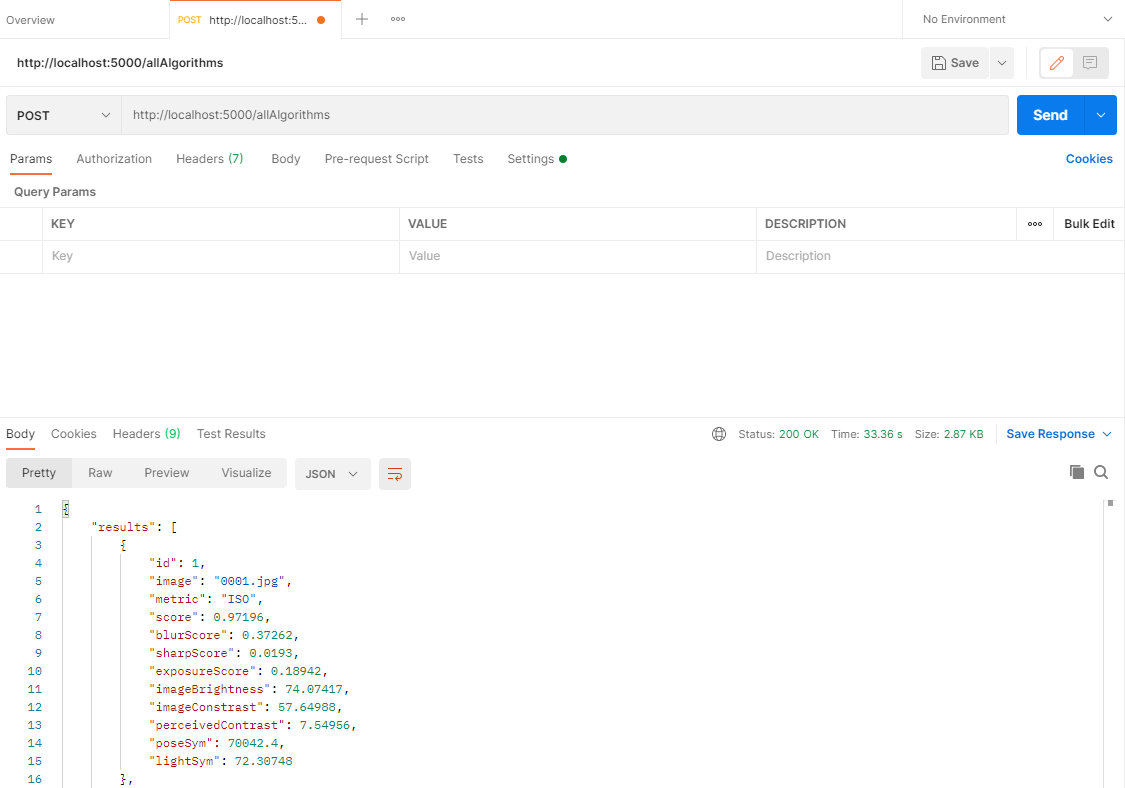
\includegraphics[scale=0.29]{figures/postman_json.PNG}
    \caption{Postman POST request}
    \label{fig:postman}
\end{figure}
%api calls implementation, adding more metrics, different routes, write to file, send file to frontend. use 3rd party software to communicate with the backend 

\subsection{Deployment}
One of the main requirements given by Mobai was to deploy the application in containers. Containerization \cite{Containerization} provided us with several benefits:
\begin{itemize}
    \item A container is independent of the operating system, making it portable between dissimilar platforms. 
    \item Containers are efficient in terms of allowing applications to quickly be deployed, patched or scaled. 
    \item Containers consume less system overhead than regular hardware or virtual environments owing to the fact that they do not include operating system images. 
    \item It provides better application development, production cycles and testing as containers supports an agile workflow.
    \item Having the application separated into different containers will improve security. 
\end{itemize}
Once functionality for the application were mostly fulfilled, the task was to package it up into two separate containers - one for the frontend and one for the backend. The basis of containers, images, were created using dockerfiles. Information that automated the application running process was stored inside the dockerfiles. That was information such as the base Docker image to run from (i.e., based on Alpine since the application was built in python), location to project code, dependencies that the application had and which commands to run at start-up. When both dockerfiles were written, the command ``Docker build'' produced two disparate images. To enable both images to run together in a remote environment, we needed to use the Docker compose tool. We created a compose file which included the definition of services that built the application. The command ``Docker compose-up'' ran the application from our compose configuration file making the images become containers running on Docker engine.

\section{Sequence diagrams}
Two sequence diagrams, one high level and one low level, will be showcased and discussed. Our web application is simple in design, but behind the scenes several entities are interacting with each other. To firmly understand how the application is constructed, it is essential to acknowledge the interaction between the components. Sequence diagrams are convenient, easy to read tools to visualize a given interaction within a time sequence. Providing both high and low level sequence diagrams will yield a complete picture of our system from a surface to an in-depth level.

\subsection{High level - ISO metric}

\begin{figure}[h]
    \centering
    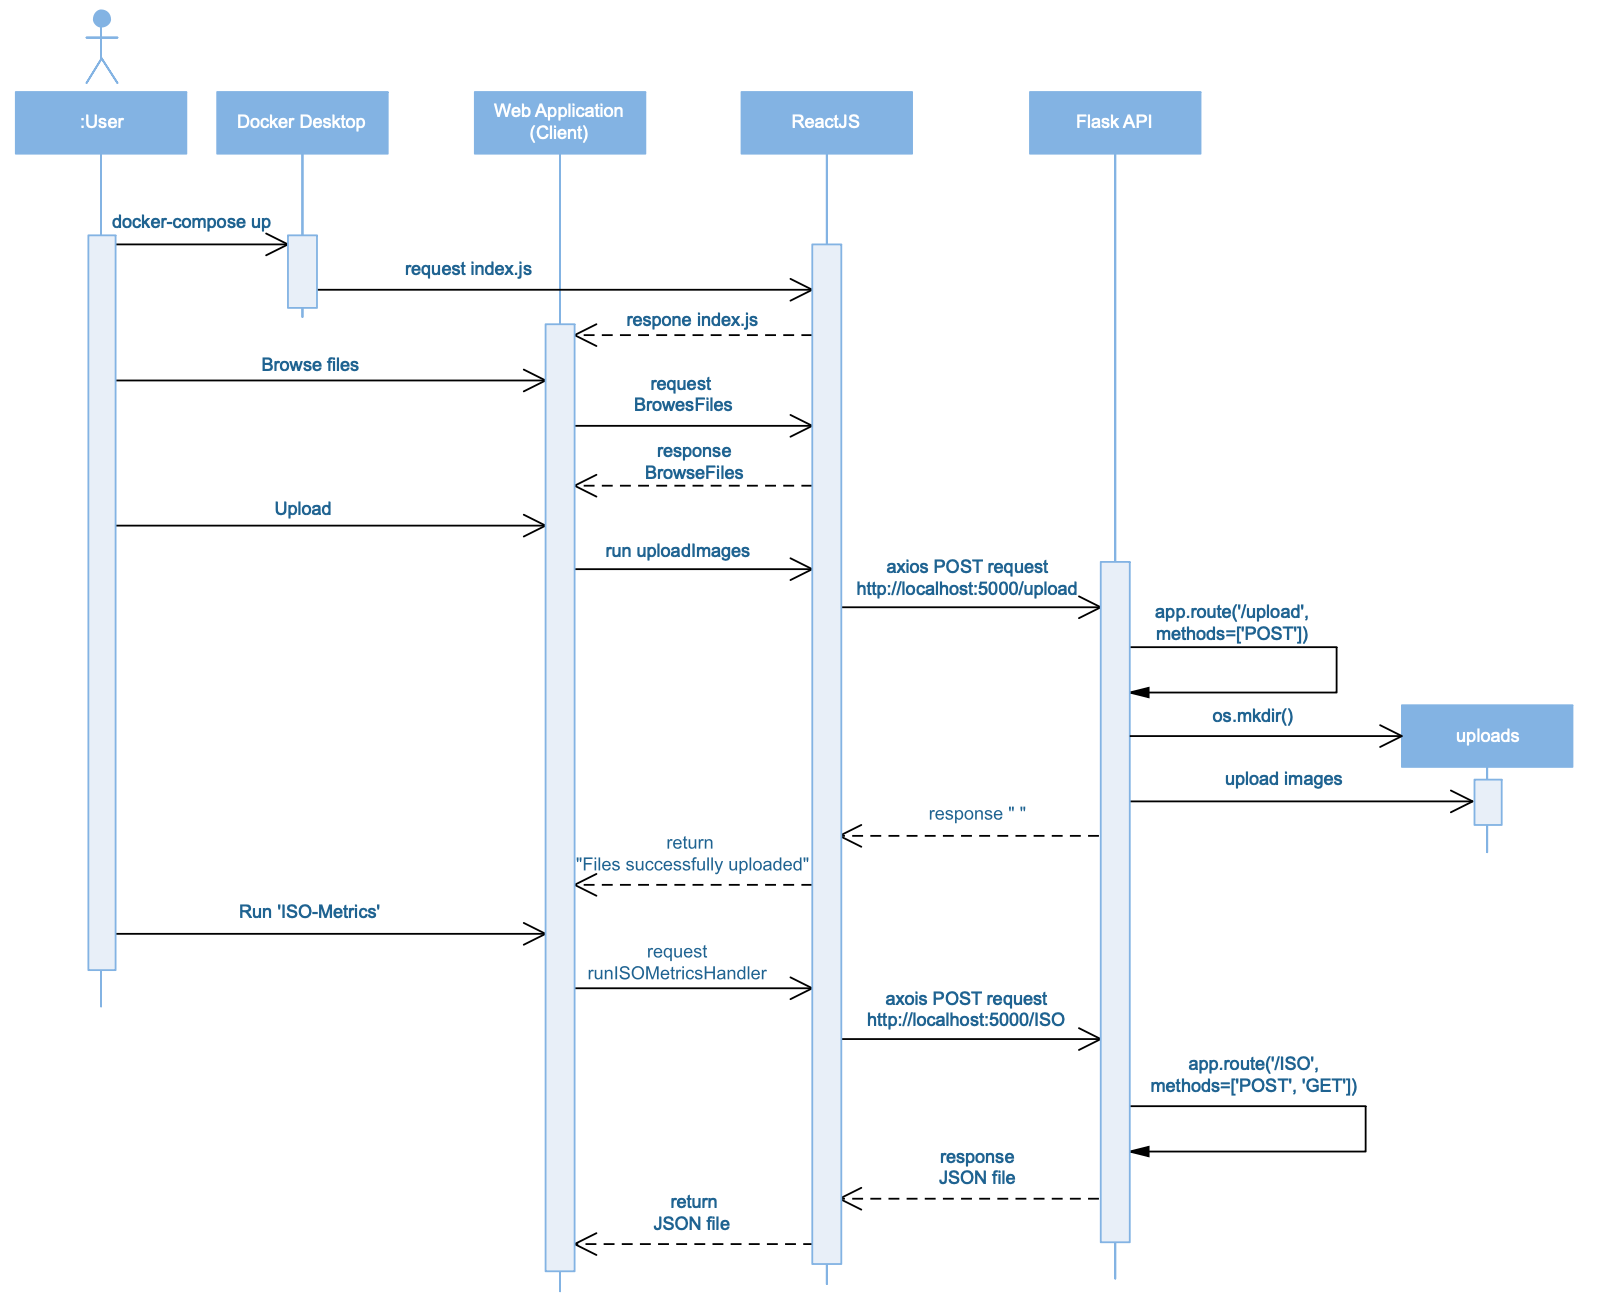
\includegraphics[scale = 0.52]{figures/HighLevel.png}
    \caption{ISO metric: high level sequence diagram}
    \label{fig:highlevel}
\end{figure}
\newpage
Figure \ref{fig:highlevel} is meant as a surface level visualization of what happens the first time the web application is started on a new computer and a metric is executed. After the two docker images are built, the application is now ready to run. From the terminal window, the command: ``docker-compose up'', will boot up both the React and Flask servers. An immediate request to render the index.js file in the web application is sent to the React server. After the home page is displayed in the web browser, the user can press a button to browse files, which will send a request to the React server to open a window of your local files. Images are now ready to be selected. The selected images are stored in a state that waits for the ``Upload'' button to be pressed. Once the user presses the button, a function called uploadImages will be executed from the React server that in return redirects an Axios HTTP POST request to the external flask backend API at port 5000. The POST request contains all the selected images. An API by the name of ``upload'' saves all selected images in a specified uploads folder in the backend before it is redirected back to the React server that displays a ``Files successfully uploaded'' message to the web application. Since this is the first time the application is executed, the uploads folder has not yet been created. The upload API therefore has to create it before uploading the images and returning to the web application. 

Once the images are saved in the backend, the web application is now ready to execute any metric. The button ``Run `ISO-Metrics''' on the web page is clicked which requests the function runISOMetricsHandler to be executed on the React server. This function will likewise redirect an Axios POST request to port 5000. An API by the name of ISO will receive the request which triggers the API to execute ISO-metric. Once the metric has generated quality scores on the uploaded images, it returns a single JSON file that contains the scores. This JSON file is returned to the React server which in return displays the scores on the web page. 
\newpage

\subsection{Low level - FaceQnet}

\begin{figure}[h]
    \centering
    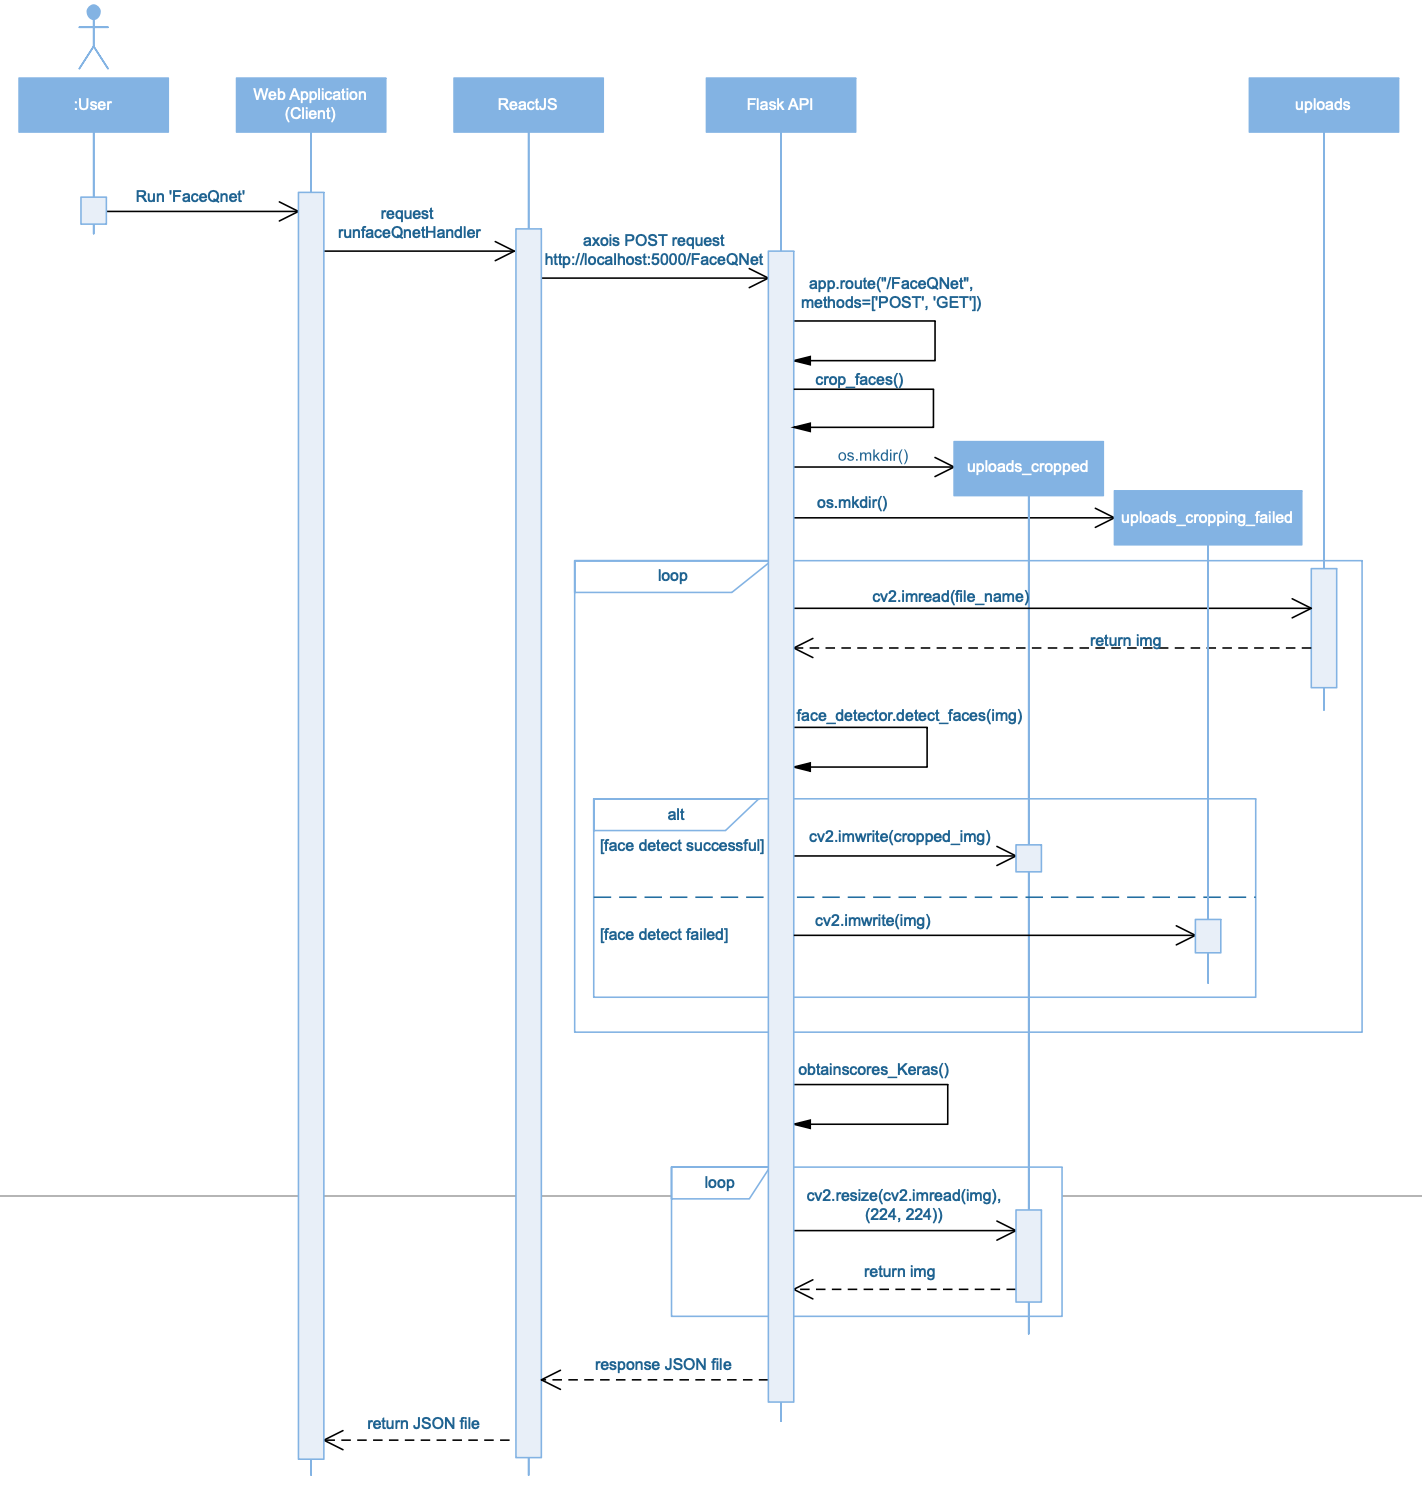
\includegraphics[scale = 0.55]{figures/FerdigLowLevel.png}
    \caption{FaceQnet: low level sequence diagram}
    \label{fig:lowlevel}
\end{figure}

Unlike Figure \ref{fig:highlevel}, Figure \ref{fig:lowlevel} in-depth showcases how FaceQnet is executed the first time it is run on a computer. Before the ``Run 'FaceQnet''' button is clicked, it is given that images have been selected and uploaded to the uploads folder, which is shown in Figure \ref{fig:highlevel}. For that reason, the ``uploads'' folder already exists instead of being created along the way. The first few steps are quite similar to the sequence diagram depicted in Figure \ref{fig:highlevel}, however this time an API called FaceQnet is executed that in return starts the FaceQnet FIQM. 
\newpage

The cropping phase of FaceQnet begins, and since this is the first time the API has been called, two folders by the name of ``uploads\_cropped'' and ``uploads\_cropping\_failed'' are created. The function then enters a for-loop that reads all the uploaded images from the original uploads folder, before they are cropped. Unfortunately, the cropping tool provided by MTCNN sometimes fails to detect the face in the images which results in an empty image. An alternative scenario then occurs, which sends these images to ``uploads\_cropping\_failed'', and they will automatically be provided with the lowest score possible. If no exception happens during the face cropping, the cropped image is saved to the uploads\_cropped folder.  

After having finished the cropping, the API starts the scores calculation, which first has to read all images from ``uploads\_cropped'', resize them and then calculates their scores. The metric likewise returns a JSON file with all scores back to the web page. 

\section{Testing}
Before we finalized the development of the web application, it was important to have the users and the product owner test the product and provide their feedback. 

\subsection{User testing}
We began the user testing at the end of the development process. The user testing was done by only one user: the product owner. The user received an email with a link to the Github repository containing the source code of the web application. The email also included a list of tasks for the user to complete and a few questions about the user experience. The tasks and questions are listed in Table \ref{table:usertesttasks} and \ref{table:usertestquestions}. The user testing was discussed with the product owner during our final meeting to expand upon the feedback we received. If there was no comment on the task or question, the feedback was set as ``satisfactory''. The required changes were later implemented to the web application.

\newpage

\begin{table}[H]
%\centering
\caption{User testing tasks and feedback}
\resizebox{\textwidth}{!}{%
\begin{tabular}{|p{7cm}|p{7cm}|} 
\hline
\textbf{Task} & \textbf{Feedback}  \\ \hline
Launch the frontend and the backend on the users' computers using Docker.
&
Satisfactory
\\ \hline
Upload multiple images to the backend from the users' computers using the frontend.
&
Satisfactory
\\ \hline
Run all metrics at the same time with the images uploaded in the second task.
&
Satisfactory
\\ \hline
Run each of the metrics separately with the images uploaded in the second task. 
&
Satisfactory
\\ \hline
Delete the images uploaded to the backend.
&
Satisfactory
\\ \hline
Upload a single image to the backend from the users' computers using the frontend.
&
Satisfactory
\\ \hline
Run all metrics at the same time with the image uploaded in the sixth task.
&
Satisfactory
\\ \hline
Run each of the metrics separately with the image uploaded in the sixth task.
&
Satisfactory
\\ \hline
\end{tabular}%
}
\label{table:usertesttasks}
\end{table}

\begin{table}[H]
\centering
\caption{User testing questions and feedback}
\resizebox{\textwidth}{!}{%
\begin{tabular}{|p{5cm}|p{9cm}|} 
\hline
\textbf{Question} & \textbf{Feedback}  \\ \hline
How is the visual design?
&
The design looks good enough. Designers can update it later to make it better.
\\ \hline
Is the user interface intuitive?
&
The user interface is simple and easy to understand.
\\ \hline
Are the metric results displayed in a satisfying way?
&
Cut down the precision of the scores from the metrics down to four digits after the decimal.

FaceQnet does not return any attribute scores and instead sets them to the number zero. This can create misunderstandings for the users. Change this to the text ``None''. Another solution is to set the score to the number minus one and add the text ``-1 indicates this approach does not return a score'' to the frontend.    
\\ \hline
Any other feedback about the user experience?
&
A loading circle is shown when the metrics are working in the backend. Add the text ``Processing is ongoing'' to let the user know what is going on.

The ``Delete'' button is located to the left of the ``Browse Files'' button. Move this to the right side of the ``Upload'' button.

Some of the text in the headers of the web application is wrapping to a new line. Keep it on the same row.
\\ \hline
\end{tabular}%
}
\label{table:usertestquestions}
\end{table}